\documentclass[border=10pt]{standalone}

\usepackage{tikz}
\usepackage{tikzsymbols}
\usetikzlibrary{calc,patterns,shapes.geometric}

\def\centerarc[#1](#2)(#3:#4:#5){\draw[#1] ($(#2)+({#5*cos(#3)},{#5*sin(#3)})$) arc (#3:#4:#5);}

\begin{document}
	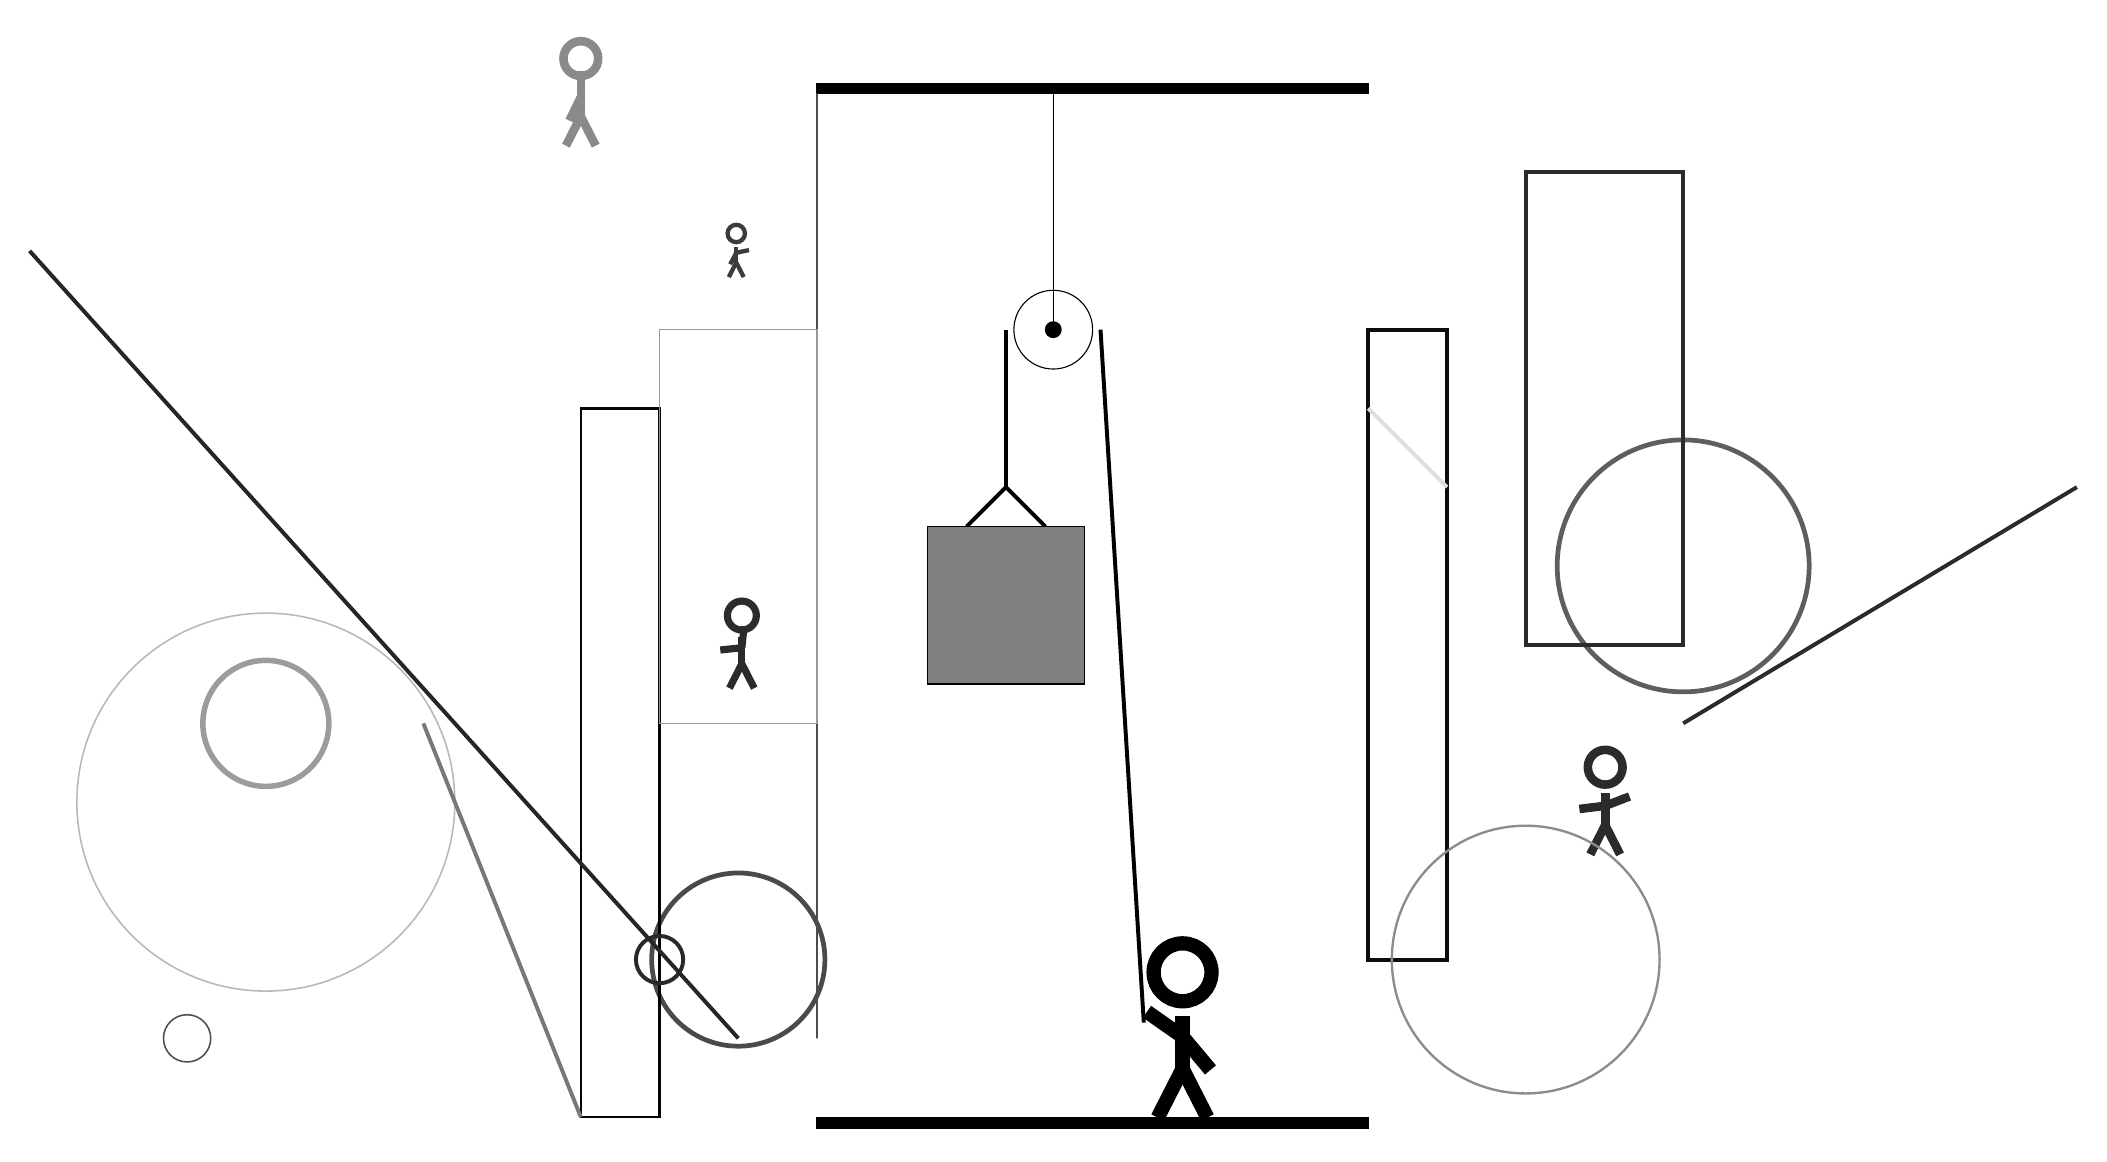
\begin{tikzpicture}
		%%%%% START %%%%%
		
		\draw[fill=black] (-2, 10) rectangle (5, 10.125);
		
		\draw (1, 7) circle (0.5);
		\draw[fill=black] (1, 7) circle (0.1);
		\draw (1, 10) -- (1, 7);
		
		\draw[line width=0.5mm] (-0.1, 4.5) -- (0.4, 5.0) -- (0.9, 4.5);
		\draw[fill=black!50] (-0.6, 4.5) rectangle (1.4, 2.5);
		
		\draw[line width=0.5mm] (0.4, 7) -- (0.4, 5.0);
		\centerarc[line width=0.5mm](1, 7)(0:180:0.6);
		\draw[line width=0.5mm](1.6, 7) -- (2.15, -1.8);
		
		\node at (2.6, -1.9) {\Strichmaxerl[10][-35][-50]};
		
		\draw [line width=0.2mm, color=black!28](-9, 1) circle (2.4);
		
		\draw [line width=0.2mm, color=black!69](-10, -2) circle (0.3);
		\node[line width=0.2mm, color=black!83] at (8, 1) {\Strichmaxerl[6][7][21]};
		\node[line width=0.5mm, color=black!83] at (-3, 3) {\Strichmaxerl[5][6][84]};
		\draw [line width=0.6mm, color=black!71](-3, -1) circle (1.1);
		\draw[line width=0.5mm, color=black!95] (6, -1) rectangle (5, 7);
		\draw [line width=0.3mm, color=black!45](7, -1) circle (1.7);
		
		\draw[line width=0.3mm, color=black!98] (-4, -3) rectangle (-5, 6);
		\draw[line width=0.5mm, color=black!13](6, 5) -- (5, 6);
		\draw[line width=0.2mm, color=black!70] (-2, -2) rectangle (-2, 10);
		\draw [line width=0.5mm, color=black!84](-4, -1) circle (0.3);
		\draw[line width=0.5mm, color=black!83](9, 2) -- (14, 5);
		\node[line width=0.2mm, color=black!46] at (-5, 10) {\Strichmaxerl[6][64][90]};
		
		\draw [line width=0.7mm, color=black!39](-9, 2) circle (0.8);
		\draw [line width=0.6mm, color=black!63](9, 4) circle (1.6);
		\node[line width=0.3mm, color=black!77] at (-3, 8) {\Strichmaxerl[3][62][12]};
		\draw[line width=0.5mm, color=black!53](-5, -3) -- (-7, 2);
		\draw[line width=0.5mm, color=black!85](-3, -2) -- (-12, 8);
		\draw[line width=0.2mm, color=black!40] (-2, 7) rectangle (-4, 2);
		\draw[line width=0.5mm, color=black!83] (7, 9) rectangle (9, 3);
		
		\draw[fill=black] (-2, -3) rectangle (5, -3.15);
		
		%%%%% END %%%%%
	\end{tikzpicture}
\end{document}